
\documentclass[11pt,a4paper]{article}
\usepackage{graphicx}
\usepackage{float}
\usepackage{titlesec}
\usepackage{fancyhdr}
\usepackage{xcolor}
\usepackage[T1]{fontenc} 
\usepackage{nameref}
\pagestyle{fancy}
\setcounter{secnumdepth}{4}
\setcounter{tocdepth}{4}
\fancyfoot[C]{\thepage}
\fancyfoot[L,R]{}
\fancyhead[C]{}
\fancyhead[L]{BearChess GUI}
\fancyhead[R]{Version 0.4.1.0}
\title{Chess GUI with support for electronic chessboards}
\author{Lars Nowak}
\date{13.03.2021} 

\begin{document}
\maketitle

\begin{abstract}
\textbf{Why yet another chess GUI?}\\

Many GUIs support electronic chessboards, but do not use the full potential that chessboards with piece recognition offer. They could be much better used for training or analysis of games and positions. Read more in chapter \textbf{\ref{AnalyzeMode}  \nameref{AnalyzeMode}} on page \pageref{AnalyzeMode}.

Another feature is the extended engine support. Read more in chapter \textbf{\ref{ExtendedSupport}  \nameref{ExtendedSupport}} on page \pageref{ExtendedSupport}.

So the focus of BearChess is more on exploiting the possibilities of the chessboards than being just another GUI. Of course, you not need an electronic chessboard to use BearChess.

The first version of BearChess supports the chessboards from Certabo and the boards connected via Millennium ChessLink.\\

As you can see from the version number, this software is still under development. There are still some functions that are not fully implemented and there are certainly still many bugs. But BearChess has now reached a level where it can be used and feedback from other users is welcome.\\

Some functions are marked with a {\color{red}\textbf{*}}. These functions are still under development.\\

I am a professional programmer and write the software in my spare time and it is free. I am not an employee of Inventhio Srl trading (Certabo) or Millennium 2000 GmbH. If something does not work, Certabo or Millennium is not responsible for it.\\

Send errors, comments, suggestions for improvement or requests to lars@solanosoft.com.

\end{abstract}

\newpage
\tableofcontents
\newpage


\section{Quick start}
\begin{itemize}
	\item Simply unpack the file BearChessWin.zip into a new folder.
	\item Start BearChess with a double-click on BearChessWin.exe
	\item Connect your electronic chessboard to your computer.
	\item Set all chessmen to their start position.
	\item Configure the electronic chessboard connection (\textbf{\ref{ElectronicChessBoard}  \nameref{ElectronicChessBoard}} on page \pageref{ElectronicChessBoard}).
	\item Connect to the electronic chessboard.
	\item Load a chess engine (\textbf{\ref{InstallEngine}  \nameref{InstallEngine}} on page \pageref{InstallEngine})
	\item Start a game and make your first move on the eletronic chessboard.
\end{itemize}

\section{Introduction}
BearChess offers among others the following functions:
\begin{enumerate}
	  \item Play with Certabo chessboards.
	  \item Play with Millennium chessboards via ChessLink modul.
  	  \item Play against human beings or UCI engines.
  	  \item Analyze your games or trainings with the help of electronic chessboards.
  	  \item Use multiple chess engines at the same time for playing and analyzing.
  	  \item Support for Polyglot and Arena opening books.
  	  \item Save and load your games
  	  \item Individual chessmen and board fields.
\end{enumerate}

BearChess follows the design of Single Document Interface (SDI). You can place different windows, e.g. chess engine output or chess move list, anywhere on your Windows desktop. If you close them or exit BearChess, the position is saved and set to the same position when reopening.


\subsection{Modes}
BearChess is running in different modes. The current mode is displayed in the lower left corner.
\begin{itemize}
	
	\item \textbf{Easy playing} This is the mode in the beginning. You just can simply start making your moves on the screen or on your electronic chessboard, almost without regard to the chess rules. In addition to support you can start chess programs or load opening books. But these only give hints, but do not play as opponents. This mode is automatically set if you are not playing in another mode. It is similar to the analyze mode but let you more easily start a new game from any position.
	\begin{figure}[H]
		\centering
		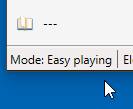
\includegraphics[scale=1.0]{ModeEasyPlaying.png}
		\caption{Easy playing}
		\label{fig:ModeEasyPlaying}
	\end{figure}
	\item \textbf{Playing a game} This is the mode if you play against a chess engine or another player. Only valid chess moves are allowed and the game is time controlled.
	\begin{figure}[H]
		\centering
		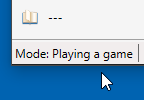
\includegraphics[scale=1.0]{ModePlayingAGame.png}
		\caption{Playing a game}
		\label{fig:ModePlayingAGame}
	\end{figure}
	\item \textbf{Analyzing} If you select this mode you can make any chess moves or place the pieces as you like, almost without regard to the chess rules. This mode is recommended to analyze a game or positions. Try different variants on the board and let several chess programs analyze the positions simultaneously. 
	\begin{figure}[H]
		\centering
		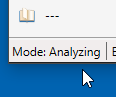
\includegraphics[scale=1.0]{ModeAnalyzing.png}
		\caption{Analyzing}
		\label{fig:ModeAnalyzing}
	\end{figure}
	\item \textbf{Setup Position} Build up a new starting position on the chessboard. It is easiest to set it up on the electronic chessboard.
	\begin{figure}[H]
		\centering
		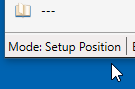
\includegraphics[scale=1.0]{ModeSetupPosition.png}
		\caption{Setup Position}
		\label{fig:ModeSetupPosition}
	\end{figure}
\end{itemize}


\section{Main window}

The first start of BearChess shows the following main window:
\begin{figure}[H]
	\centering
	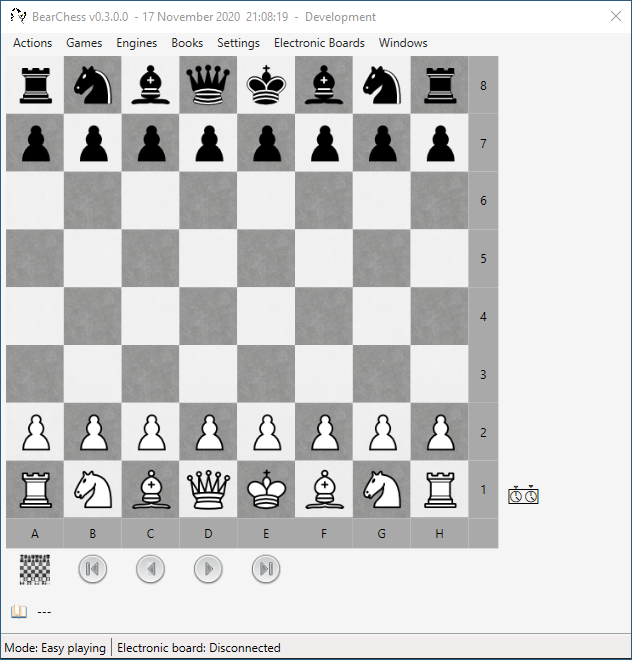
\includegraphics[scale=0.8]{BearChess_MainWindow.png}
	\caption{Main window}
	\label{fig:MainWindow}
\end{figure}

Two buttons are active:
\begin{itemize}
  \item 
\includegraphics[scale=0.5]{arrow_rotate_anticlockwise.png} rotates the board.
  \item 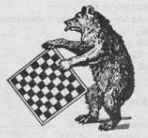
\includegraphics[scale=0.2]{bearchess_2.png} is an easy way to play a game.
Read more in chapter \textbf{\ref{easyStart}  \nameref{easyStart}} on page \pageref{easyStart}.
\end{itemize}



\subsection{Actions}
\begin{figure}[H]
	\centering
	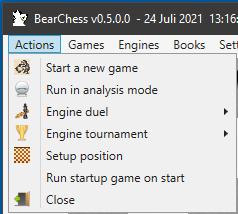
\includegraphics[scale=1.0]{Actions.png}
	\caption{Actions}
	\label{fig:Actions}
\end{figure}
\begin{itemize}
	\item 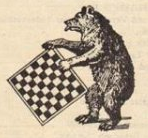
\includegraphics[scale=0.2]{bearchess.png} \textbf{Play a new game} opens a new window to select opponents and time control (see chapter \textbf{\ref{SelectOpponent}  \nameref{SelectOpponent}} on page \pageref{SelectOpponent}).
	\item 
\includegraphics[scale=0.5]{robot.png} \textbf{Run in analyze mode} allows you to analyze games or positions with suppport of several chess engines (see chapter \textbf{\ref{AnalyzeMode}  \nameref{AnalyzeMode}} on page \pageref{AnalyzeMode})
	\item 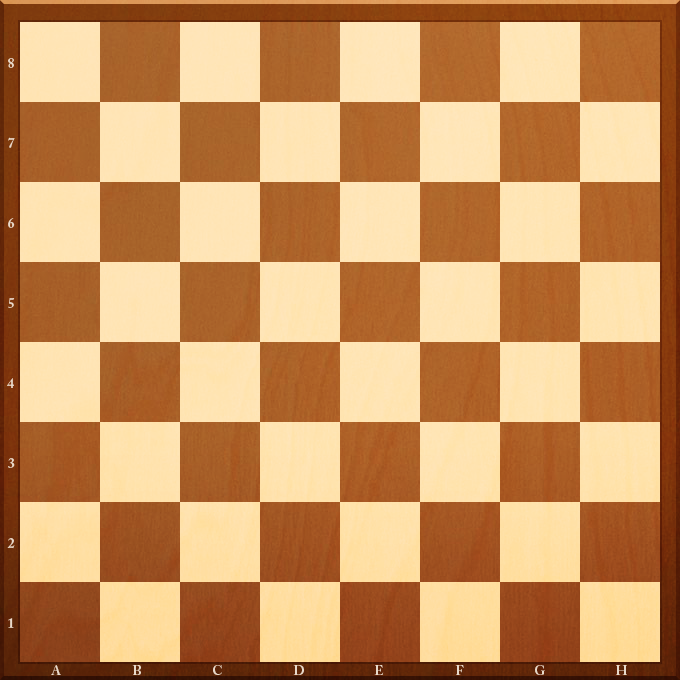
\includegraphics[scale=0.03]{Chess_Board.png} see chapter \textbf{\ref{SetupPosition}  \nameref{SetupPosition}} on page \pageref{SetupPosition}.
	\item \textbf{Run startup game on start} immediately starts a new game when you start BearChess. For more information read chapter \textbf{\ref{startupgame}  \nameref{startupgame}} on page \pageref{startupgame}.
	\item 
\includegraphics[scale=0.5]{door_out.png} \textbf{Close} exits BearChess.
\end{itemize}

\subsection{Games}
\begin{figure}[H]
	\centering
	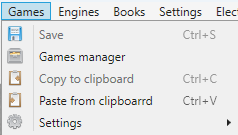
\includegraphics[scale=1.0]{Games1.png}
	\caption{Games}
	\label{fig:Games}
\end{figure}
\begin{itemize}
	\item 
\includegraphics[scale=0.5]{diskette.png} \textbf{Save} your current game.
	\item 
\includegraphics[scale=0.5]{file_manager.png}  \textbf{Show \& Load} opens a new window in which you can see and load all your previously saved games.
	\item 
\includegraphics[scale=0.5]{clipboard_sign.png}  \textbf{Paste from clipboard} loads a game (PGN) from your clipboard.
\end{itemize}
All games are saved in a database file. Read more on chapter \textbf{\ref{games}  \nameref{games}} on page \pageref{games}.

\subsection{Engines}
\begin{figure}[H]
	\centering
	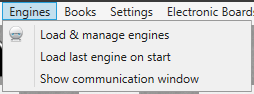
\includegraphics[scale=1.0]{Engines.png}
	\caption{Engines}
	\label{fig:Engines}
\end{figure}
\begin{itemize}
	\item  
\includegraphics[scale=0.5]{robot.png} \textbf{Load \& manage engines} opens a new window in which you can install, load or configure your chess engines.
	\item \textbf{Load last engine on start} if you always want to load immediately an engine when you start BearChess. It has no effect if you have activated the option "Run startup game on start".
	\item \textbf{Show communication window} opens a new window where you can follow the communication between BearChess and chess engines. It is useful to detect any problems in communication.
	\item \textbf{Settings} to configure if you want to see more information from the engine, e.g. nodes per second.	
\end{itemize}

Read more on chapter \textbf{\ref{loadEngines}  \nameref{loadEngines}} on page \pageref{loadEngines}.

\subsection{Books}
\begin{figure}[H]
	\centering
	\includegraphics[scale=1.0]{Books.png}
	\caption{Books}
	\label{fig:Books}
\end{figure}
\begin{itemize}
	\item 
\includegraphics[scale=0.5]{books_stack.png} \textbf{Load \& manage opening books} opens a new window in which you can install or load  your opening books.
\end{itemize}
BearChess can handle Polyglot and Arena opening books. Read more on chapter \textbf{\ref{OpeningBooks}  \nameref{OpeningBooks}} on page \pageref{OpeningBooks}.

\subsection{Settings}
\begin{figure}[H]
	\centering
	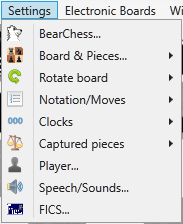
\includegraphics[scale=1.0]{Settings.png}
	\caption{Settings}
	\label{fig:Settings}
\end{figure}
\begin{itemize}
	\item  
\includegraphics[scale=0.9]{Board2DPieces32.png} \textbf{Board \& Pieces} opens a window where you can change the appearance of the chessboard and the pieces.  Read more on chapter \textbf{\ref{BoardAndPieces}  \nameref{BoardAndPieces}} on page \pageref{BoardAndPieces}.
	\item 
\includegraphics[scale=0.5]{arrow_rotate_anticlockwise.png}  \textbf{Rotate board} if the board on the screen should automatically rotate for your color.
	\item  
\includegraphics[scale=0.5]{text_list_numbers.png} \textbf{Notation/Moves} opens a windows where you can change the appearance of the notation, e.g. figurine or letters.
	\item  
\includegraphics[scale=0.5]{digit_separator.png}  \textbf{Clocks} switches between large and small clocks.
	\item  
\includegraphics[scale=0.5]{balance_unbalance.png}  \textbf{Captured pieces} shows the captured pieces window at startup or on demand.
\end{itemize}

\subsection{Electronic Boards}
\begin{figure}[H]
	\centering
	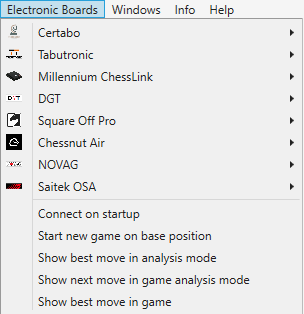
\includegraphics[scale=1.0]{ElectronicBoards.png}
	\caption{Electronic Boards}
	\label{fig:ElectronicBoards}
\end{figure}
\begin{itemize}
	\item  
\includegraphics[scale=0.1]{Certabo_icon.png} \textbf{Certabo} opens a window where you can configure and connect to Certabo chessboards.  Read more on chapter \textbf{\ref{ConfigureCertabo}  \nameref{ConfigureCertabo}} on page \pageref{ConfigureCertabo}.
	\item  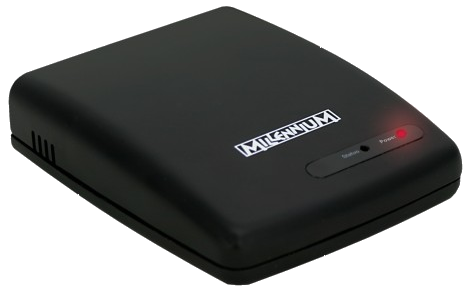
\includegraphics[scale=0.05]{Millennium ChessLink.png} \textbf{Millennium ChessLink} opens a window in which you can configure chessboards connected to Millennium ChessLink and connect to them.  Read more on chapter \textbf{\ref{ConfigureChessLink}  \nameref{ConfigureChessLink}} on page \pageref{ConfigureChessLink}.
	\item \textbf{Connect on startup} tries to connect on to the last connected chessboard when BearChess is started. 	
	\item \textbf{Black pieces in front} assumes that you have placed the black chessmen in front of you.
	\item \textbf{Start a new game on base position} recognizes when you reset all the pieces to the base position during a game. In this case, a new game will be started automatically.
\end{itemize}

\subsection{Windows}
\begin{figure}[H]
	\centering
	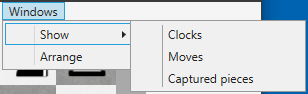
\includegraphics[scale=1.0]{Windows.png}
	\caption{Windows}
	\label{fig:Windows}
\end{figure}
\begin{itemize}
	\item \textbf{Show} brings clocks or move list windows to the foreground if they are currently not visible.
	\item \textbf{Arrange} auto arange all windows to fit on your screen and not overlapping.
	\item \textbf{Captured pieces} shows the captured pieces. Either all or as a difference. 
\end{itemize}

\section{Install, Configure and Load a chess engine} \label{loadEngines}

\begin{figure}[H]
	\centering
	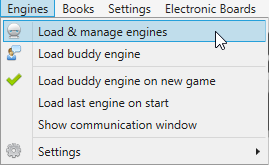
\includegraphics[scale=1.0]{LoadEngine.png}
	\caption{Open Load And Manage UCI Engines window}
	\label{fig:LoadEngine}
\end{figure}
BearChess does not include a chess engine. Click on "Load \& manage engines" to install and configure one. "\textit{Install}" means to make a chess program BearChess known, not to install it on your computer. BearChess supports any UCI engine.\\
\begin{figure}[H]
	\centering
	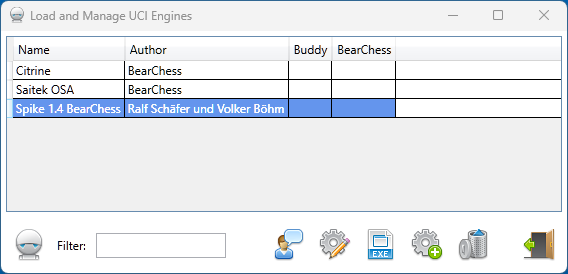
\includegraphics[scale=1.0]{LoadManageEngine1.png}
	\caption{Load And Manage UCI Engines}
	\label{fig:LoadManageEngine1}
\end{figure}

\begin{itemize}
	\item 
\includegraphics[scale=0.5]{robot.png} Load selected engine
	\item 
\includegraphics[scale=0.5]{cog.png} Configure selected engine
	\item 
\includegraphics[scale=0.5]{file_extension_exe.png} Install a new engine
	\item 
\includegraphics[scale=0.5]{bin.png} Uninstall selected engine
	\item 
\includegraphics[scale=0.5]{door_out.png} Close the window
\end{itemize}

\subsection{Install a new engine} \label{InstallEngine}

To install a new engine click on 
\includegraphics[scale=0.5]{file_extension_exe.png} and select an UCI engine file, e.g. the latest Stockfish exe file. Or you just drag \& drop the exe file onto the button.
\begin{figure}[H]
	\centering
	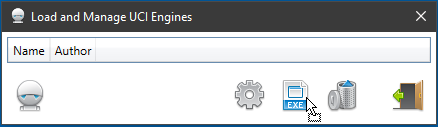
\includegraphics[scale=1.0]{DropEngine.png}
	\caption{Drop an engine file}
	\label{fig:DropEngine}
\end{figure}

 If the file detected as UCI engine, confirm your selection.\\
Next, a configuration dialog box appears where you can configure the engine and give it a name.
\begin{figure}[H]
	\centering
	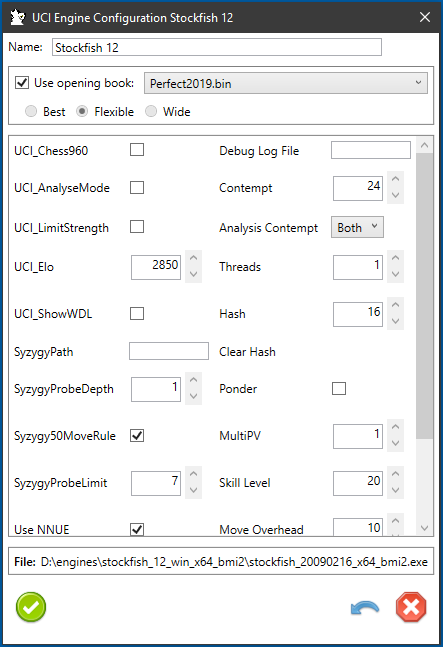
\includegraphics[scale=0.8]{ConfigureStockfish.png}
	\caption{Engine configuration}
	\label{fig:ConfigureStockfish}
\end{figure}
The name is freely assignable, must be unique across all engines. But this way you can install the same engine several times with different configurations. The configuration values, names and possibilities are given by the engines. The first time these are the default values.
\begin{itemize}
	\item 
\includegraphics[scale=0.5]{accept_button.png} Accept the changes
	\item 
\includegraphics[scale=0.5]{undo.png} Reset to default values
	\item 
\includegraphics[scale=0.5]{cancel.png} Cancel
\end{itemize}
The small 
\includegraphics[scale=0.3]{folder.png} button opens a file or directory selection dialog, depending on the configuration name (file, path, dir).\\
The configuration type 'button', e.g. 'Clear Hash', works only if the engine is loaded.

\subsubsection{Use opening book}
Some engines comes with there own opening book and you have an option to use them or not. You can also tell BearChess to use an opening book before the moves are calculated by the engines. You can configure how BearChess determines the book move. 
\begin{itemize}
	\item \textbf{Best} Always chooses the best move
	\item \textbf{Flexible} Selects one of the best moves
    \item \textbf{Wide} Selects any book move
\end{itemize}
Look at chapter \textbf{\ref{OpeningBooks}  \nameref{OpeningBooks}} on page \pageref{OpeningBooks} how to install an opening book.


\subsection{Configure an engine}

To change the configuration of an installed engine click on 
\includegraphics[scale=0.5]{cog.png}\\
The same configuration dialog box as during installation is shown where you can configure the engine or just change the name.

\subsection{Additional configuration for an installed engine}

If you want to save the same program with a different configuration, e.g. an additional configuration with adjusted Elo strength, you can save the configuration under a different name.

\begin{figure}[H]
	\centering
	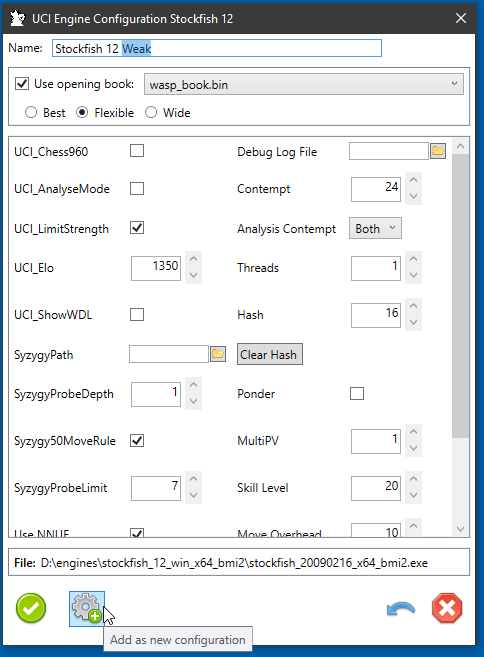
\includegraphics[scale=0.8]{ConfigureStockfish_2.png}
	\caption{Save as new configuration}
	\label{fig:LoadEngine3}
\end{figure}
Click on 
\includegraphics[scale=0.5]{cog_add.png} to save the configuration with a new name.\\


\subsection{Load an engine}

To load an installed engine, select an engine and click on 
\includegraphics[scale=0.5]{robot.png} or just double-click.

\begin{figure}[H]
	\centering
	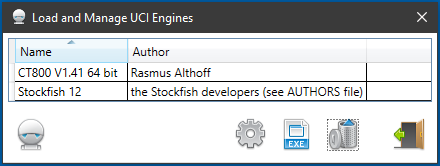
\includegraphics[scale=1.0]{LoadEngine2.png}
	\caption{Some installed engines}
	\label{fig:LoadEngine2}
\end{figure}

\section{Load and Manage Opening Books} \label{OpeningBooks}

\begin{figure}[H]
	\centering
	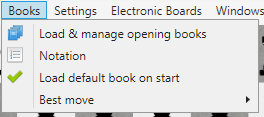
\includegraphics[scale=1.0]{books.png}
	\caption{Open Load and Manage Opening Books  }
	\label{fig:LoadManageBooks1}
\end{figure}

BearChess does not include opening books. Click on "Load \& manage opening books" to install one. "\textit{Install}" means to make a opening book BearChess known, not to install it on your computer. BearChess supports Polyglot and Arena opening books.\\

\begin{figure}[H]
	\centering
	\includegraphics[scale=1.0]{LoadManageBooks2.png}
	\caption{Load and Manage Opening Books  }
	\label{fig:LoadManageBooks2}
\end{figure}

\begin{itemize}
	\item \includegraphics[scale=0.5]{book_open.png} Load selected book
	\item \includegraphics[scale=0.5]{book_add.png} Install a new book
	\item \includegraphics[scale=0.5]{bin.png} Uninstall selected book
	\item \includegraphics[scale=0.5]{door_out.png} Close the window
\end{itemize}

To install a new opening book click on \includegraphics[scale=0.5]{book_add.png} and select a book file. The file extension for Polyglot books is \textbf{bin} and for Arena is \textbf{abk}.

\begin{figure}[H]
	\centering
	\includegraphics[scale=1.0]{LoadManageBooks3.png}
	\caption{Some installed books }
	\label{fig:LoadManageBooks3}
\end{figure}

To select an opening book click on \includegraphics[scale=0.5]{book_open.png} or just double-click. 
A new window opens and shows the current possible moves found in the book.

\begin{figure}[H]
	\centering
	\includegraphics[scale=1.0]{OpeningBook.png}
	\caption{Loaded opening book on base position }
	\label{fig:OpeningBook}
\end{figure}

You can load more than one book. Every book has their own window and is synchronized with the current position on the chessboard.

\begin{figure}[H]
	\centering
	\includegraphics[scale=0.8]{OpeningBook2.png}
	\caption{Loaded opening books }
	\label{fig:OpeningBook2}
\end{figure}

{\color{red}\textbf{*}} So far, the possibilities are still very limited with the opening books. This will improve in the next versions. 

\section{Configure Board and Pieces} \label{BoardAndPieces}

\begin{figure}[H]
	\centering
	\includegraphics[scale=1.0]{SettingsBoardAndPieces.png}
	\caption{Open window to configure board and pieces }
	\label{fig:SettingsBoardAndPieces}
\end{figure}

To change the appearance of BearChess select "Board and Pieces". A new window opens where your can configure it. BearChess comes with one set of pieces and board colors.

\begin{figure}[H]
	\centering
	\includegraphics[scale=0.9]{SettingsBoardAndPieces2.png}
	\caption{Setup board and pieces }
	\label{fig:SettingsBoardAndPieces2}
\end{figure}


\begin{itemize}
	\item \includegraphics[scale=0.5]{file_manager.png} Install new board colors or pieces
	\item \includegraphics[scale=0.5]{bin.png} Uninstall board colors or pieces
	\item \includegraphics[scale=0.5]{accept_button.png} Accept the changes
	\item \includegraphics[scale=0.5]{cancel.png} Cancel
\end{itemize}

If the options "Show last move" and "Show best move" are activated, the last move and the currently best analysis move of an engine are marked on the board.

\begin{figure}[H]
	\centering
	\includegraphics[scale=0.8]{LastMove.png}
	\caption{Last move }
	\label{fig:LastMove}
\end{figure}


\begin{figure}[H]
	\centering
	\includegraphics[scale=0.8]{BestMove.png}
	\caption{Currently best move }
	\label{fig:BestMove}
\end{figure}

\subsection{Install new board colors and pieces}
BearChess uses png files for board colors and pieces.

\subsubsection{New board colors}
Click on \includegraphics[scale=0.5]{file_manager.png} to select a directory where the files are located. BearChess accepts \verb|w.png| or \verb|white.png| for white fields and \verb|b.png| or \verb|black.png| for black fields.

\begin{figure}[H]
	\centering
	\includegraphics[scale=1.0]{WoodPieces.png}
	\caption{Example for wood fields }
	\label{fig:WoodPieces}
\end{figure}

If BearChess find both files inside the directory it builds an empty chessboard to confirm your choice. A name for your board is required.

\begin{figure}[H]
	\centering
	\includegraphics[scale=1.0]{ConfirmBoard.png}
	\caption{Confirm new board }
	\label{fig:ConfirmBoard}
\end{figure}

\subsubsection{New pieces}
There a two ways to install a new set of pieces. One png file for each piece or one png file with all pieces inside. \\
Click on \includegraphics[scale=0.5]{file_manager.png} to select a directory where the files are located.\\ \textbf{Important:} The png files must have a transparent background color, otherwise they would paint over the fields.
BearChess accepts following names for the different pieces:
\begin{itemize}
	\item \textbf{White king:} \verb|KingW.png, WhiteKing.png, wk.png|
	\item \textbf{Black king:} \verb|KingB.png, BlackKing.png, bk.png|
	\item \textbf{White queen:} \verb|QueenW.png, WhiteQueen.png, wq.png|
	\item \textbf{Black queen:} \verb|QueenB.png, BlackQueen.png, bq.png|
	\item \textbf{White rook:} \verb|RookW.png, WhiteRook.png, wr.png|
	\item \textbf{Black rook:} \verb|RookB.png, BlackRook.png, br.png|
	\item \textbf{White bishop:} \verb|BishopW.png, WhiteBishop.png, wb.png|
	\item \textbf{Black bishop:} \verb|BishopB.png, BlackBishop.png, bb.png|
	\item \textbf{White knight:} \verb|KnightW.png, WhiteKnight.png, wn.png|
	\item \textbf{Black knight:} \verb|KnightB.png, BlackKnight.png, bn.png|
	\item \textbf{White pawn:} \verb|PawnW.png, WhitePawn.png, wp.png|
	\item \textbf{Black pawn:} \verb|PawnB.png, BlackPawn.png, bp.png|
\end{itemize}


\begin{figure}[H]
	\centering
	\includegraphics[scale=0.7]{Pieces.png}
	\caption{Example one png file for each piece}
	\label{fig:Pieces}
\end{figure}

If BearChess find all files inside the directory it builds an piece set to confirm your choice.\\

If BearChess find only one png file inside the directory it assumes that this file contains all pieces at once.

\begin{figure}[H]
	\centering
	\includegraphics[scale=6.5]{Leipzig.png}
	\caption{One png file with all pieces}
	\label{fig:Leipzig}
\end{figure}

The png must have the pieces in the order and colors shown above.\\
If you have one png file for all pieces, you can just drgp \& drop the png file onto the
open file dialog icon. It avoids the effort of having to have a separate directory for each file.
\begin{figure}[H]
	\centering
	\includegraphics[scale=0.9]{DropPieceSet.png}
	\caption{Drop new pieces }
	\label{fig:DropPieceSet}
\end{figure}

\begin{figure}[H]
	\centering
	\includegraphics[scale=0.9]{ConfirmPieces.png}
	\caption{Confirm new pieces }
	\label{fig:ConfirmPieces}
\end{figure}

BearChess builds an piece set to confirm your choice. A name for your set is required.
Now you can combine your boards with your pieces.

\begin{figure}[H]
	\centering
	\includegraphics[scale=0.8]{CombineBoardPieces.png}
	\caption{Combine board and pieces }
	\label{fig:CombineBoardPieces}
\end{figure}


\section{Configure Notation and Moves}
\begin{figure}[H]
	\centering
	\includegraphics[scale=0.9]{NotationAndMoves1.png}
	\caption{Opens a window to configure notation and moves }
	\label{fig:NotationAndMoves}
\end{figure}
BearChess can display moves in different ways.
\begin{figure}[H]
	\centering
	\includegraphics[scale=1.0]{NotationAndMoves2.png}
	\caption{Configure notation and moves }
	\label{fig:NotationAndMoves}
\end{figure}
In long and short notation and with symbols or letters for the chessmen.

\section{Configure clock style}
\begin{figure}[H]
	\centering
	\includegraphics[scale=1.0]{ConfigureClocks.png}
	\caption{Configure clocks }
	\label{fig:ConfigureClocks}
\end{figure}

BearChess offers two different clocks: small and big

\begin{figure}[H]
	\centering
	\includegraphics[scale=1.0]{SmallClocks.png}
	\caption{Small clocks }
	\label{fig:SmallClocks}
\end{figure}
\begin{figure}[H]
	\centering
	\includegraphics[scale=0.8]{BigClocks.png}
	\caption{Big clocks }
	\label{fig:BigClocks}
\end{figure}

\section{Show captured pieces}
\begin{figure}[H]
	\centering
	\includegraphics[scale=1.0]{CapturedPieces1.png}
	\caption{Show captured pieces }
	\label{fig:CapturedPieces1}
\end{figure}

Opens a window that shows the captured pieces.
\begin{figure}[H]
	\centering
	\includegraphics[scale=1.0]{CapturedPieces2.png}
	\caption{Show captured pieces on start }
	\label{fig:CapturedPieces2}
\end{figure}
You can configure this window so that it is displayed at startup.

\begin{figure}[H]
	\centering
	\includegraphics[scale=1.0]{CapturedPieces3.png}
	\caption{Show all captured pieces }
	\label{fig:CapturedPieces3}
\end{figure}

Figure \ref{fig:CapturedPieces3} shows all captured pieces. Black is one queen, one knight a two pawns ahead.

\begin{figure}[H]
	\centering
	\includegraphics[scale=1.0]{CapturedPieces4.png}
	\caption{Show captured pieces as difference}
	\label{fig:CapturedPieces4}
\end{figure}
Figure \ref{fig:CapturedPieces4} shows the same information as difference.

The button \includegraphics[scale=0.5]{balance_unbalance.png} switches between both views.


\section{Electronic chessboards} \label{ElectronicChessBoard}
BearChess supports two electronic chessboards: Certabo boards and Millennium boards via the ChessLink module. Both boards communicates via an USB port as serial COM port. Which COM port is used is not the same for all computers and can change over time, especially if you have more than one COM port available on your computer.

\subsection{Configure Certabo boards} \label{ConfigureCertabo}
\begin{figure}[H]
	\centering
	\includegraphics[scale=1.0]{Certabo1.png}
	\caption{Open a window to configure Certabo boards }
	\label{fig:Certabo1}
\end{figure}

Certabo requires two configuration steps. The used COM-port and a calibration to detect the chess pieces.

\begin{figure}[H]
	\centering
	\includegraphics[scale=1.0]{Certabo2.png}
	\caption{Configure Certabo boards }
	\label{fig:Certabo2}
\end{figure}

Select the COM port if you know them or let the <auto> selection.
Click on \includegraphics[scale=0.5]{connect.png} to verify your selection.

\begin{figure}[H]
	\centering
	\includegraphics[scale=0.9]{Calibrate1.png}
	\caption{COM port successful detected}
	\label{fig:Calibrate1}
\end{figure}

If you select an invalid COM port, you will receive the following error message:

\begin{figure}[H]
	\centering
	\includegraphics[scale=0.9]{Calibrate2.png}
	\caption{Invalid COM port }
	\label{fig:Calibrate2}
\end{figure}

If you select <auto> and no board is found, you will receive the following error message:

\begin{figure}[H]
	\centering
	\includegraphics[scale=0.9]{Calibrate3.png}
	\caption{No board found }
	\label{fig:Calibrate3}
\end{figure}

\textbf{Hint:} You can always use the selection <auto>, but if you have more than one COM port available, it can always take some seconds until the right one is recognized.

\subsubsection{Calibration}
At the first start, BearChess needs a calibration to identify your chessmen. A new calibration is only required if you use another set of chessmen.\\
Click on \includegraphics[scale=0.08]{chessboard_base.png} to open the calibration dialog.
\begin{figure}[H]
	\centering
	\includegraphics[scale=1.0]{CalibrateBase.png}
	\caption{Calibrate base position }
	\label{fig:CalibrateBase}
\end{figure}
If all pieces on the right position click the accept button. When a calibration is running, you will see the chessboard LEDs flashing each row. Please wait until all LEDs are off and the confirm dialog appears.

\begin{figure}[H]
	\centering
	\includegraphics[scale=1.0]{Calibrate4.png}
	\caption{Calibration finished }
	\label{fig:Calibrate4}
\end{figure}

\textbf{Hint:} If the calibration never seems to end, check that the chessmen are correctly placed in the middle of the squares.

\subsubsection{Connect}
\begin{figure}[H]
	\centering
	\includegraphics[scale=1.0]{Certabo3.png}
	\caption{Connect to Certabo}
	\label{fig:Certabo3}
\end{figure}
When the configuration is complete, you can connect to your chessboard.
In the lower right corner a new button appears, which allows you to easily connect or disconnect your board. The current status is also written.

\begin{figure}[H]
	\centering
	\includegraphics[scale=0.8]{Certabo4.png}
	\caption{Connected}
	\label{fig:Certabo4}
\end{figure}

\begin{figure}[H]
	\centering
	\includegraphics[scale=0.8]{Certabo5.png}
	\caption{Disconnected}
	\label{fig:Certabo5}
\end{figure}

\subsection{Configure Millennium ChessLink} \label{ConfigureChessLink}
\begin{figure}[H]
	\centering
	\includegraphics[scale=1.0]{MillenniumChessLink1.png}
	\caption{Open a window to configure Millennium boards }
	\label{fig:MillenniumChessLink1}
\end{figure}

For your Millennium ChessLink you may need to configure the COM port used. You can also change how the LEDs should light up.\\
If your PC supports Bluetooth, you can also connect to the ChessLink module via Bluetooth. If you want to do this, check the option "Bluetooth" first, before opening the configuration windows. 
\begin{figure}[H]
	\centering
	\includegraphics[scale=1.0]{MillenniumChessLink9.png}
	\caption{Search for Bluetooth }
	\label{fig:MillenniumChessLink9}
\end{figure}
Read chapter \textbf{\ref{Bluetooth}  \nameref{Bluetooth}} on page \pageref{Bluetooth} for more information.

\begin{figure}[H]
	\centering
	\includegraphics[scale=0.9]{MillenniumChessLink2.png}
	\caption{Configure Millennium ChessLink }
	\label{fig:MillenniumChessLink2}
\end{figure}

Select the COM port if you know them or let the <auto> selection.
Click on \includegraphics[scale=0.5]{connect.png} to verify your selection.

\begin{figure}[H]
	\centering
	\includegraphics[scale=0.9]{MillenniumChessLink3.png}
	\caption{COM port successful detected }
	\label{fig:MillenniumChessLink3}
\end{figure}

If you select an invalid COM port, you will receive the following error message:

\begin{figure}[H]
	\centering
	\includegraphics[scale=0.9]{MillenniumChessLink4.png}
	\caption{Invalid COM port }
	\label{fig:MillenniumChessLink4}
\end{figure}

If you select <auto> and no board is found, you will receive the following error message:

\begin{figure}[H]
	\centering
	\includegraphics[scale=0.9]{MillenniumChessLink5.png}
	\caption{No board found }
	\label{fig:MillenniumChessLink5}
\end{figure}

\textbf{Hint:} You can always use the selection <auto>, but if you have more than one COM port available, it can always take some seconds until the right one is recognized.\\

You can change how the LEDs should light up. The brightness and whether the LEDs should flash alternately or synchronously when indicating moves.

\subsubsection{Configure Bluetooth} \label{Bluetooth}

If the "Bluetooth" option is set, the following window will be displayed for a short time if you open the configuration dialog.

\begin{figure}[H]
	\centering
	\includegraphics[scale=0.8]{MillenniumChessLink10.png}
	\caption{Search for Bluetooth}
	\label{fig:MillenniumChessLink10}
\end{figure}

During this time or if you connect to the first time, Windows may ask you to connect to the Millennium ChessLink module. In this case, confirm this. Once you have successfully connected to the ChessLink module via Bluetooth, you should deactivate the "Bluetooth" option.

\subsubsection{Connect}
\begin{figure}[H]
	\centering
	\includegraphics[scale=1.0]{MillenniumChessLink6.png}
	\caption{Connect to Millennium ChessLink}
	\label{fig:MillenniumChessLink6}
\end{figure}
When the configuration is complete, you can connect to your chessboard.
In the lower right corner a new button appears, which allows you to easily connect or disconnect your board. The current status is also written.

\begin{figure}[H]
	\centering
	\includegraphics[scale=0.8]{MillenniumChessLink7.png}
	\caption{Connected}
	\label{fig:MillenniumChessLink7}
\end{figure}

\begin{figure}[H]
	\centering
	\includegraphics[scale=0.8]{MillenniumChessLink8.png}
	\caption{Disconnected}
	\label{fig:MillenniumChessLink8}
\end{figure}


\section{Play a game}

\begin{figure}[H]
	\centering
	\includegraphics[scale=1.0]{NewGame1.png}
	\caption{Opens a window to play a new game}
	\label{fig:NewGame1}
\end{figure}

If you start a new game you can select the opponents and the time control.

\subsection{Select opponent} \label{SelectOpponent}

\begin{figure}[H]
	\centering
	\includegraphics[scale=0.9]{NewGame2.png}
	\caption{Play a new game}
	\label{fig:NewGame2}
\end{figure}

Select the opponents for white \includegraphics[scale=0.4]{KingW.png} and black \includegraphics[scale=0.4]{KingB.png}. "Player" means a human opponent. You can select "Player" for white and black if you want to play a game against another human opponent on your chessboard. You can select an engine for white and black if you want to play a pure engine match.\\
\includegraphics[scale=0.4]{user_silhouette.png} is a shortcut to select "Player".\\


\textbf{Hint:} You cannot use an electronic chessboard for a pure engine match.\\

\includegraphics[scale=0.4]{cog.png} opens the engine configuration dialog. This is the same dialog as for load and manage engines. However, all changes are only used for this game and are not saved permanently.\\
Below the engine selection, there are up to three information which gives you a quick overview of the current engine configuration.

\begin{itemize}
	\item \textbf{Ponder} if the engine supports pondering, the icons \includegraphics[scale=0.4]{tick.png} and \includegraphics[scale=0.4]{delete.png} shows the current state.
	\item \textbf{Elo} if the engine supports allows to restrict the Elo performance, the current value is shown.
	\item  \includegraphics[scale=0.4]{book_open.png} for "yes" and \includegraphics[scale=0.4]{book.png} for "no" shows the current state of using an opening book.
\end{itemize}


\subsection{Start from}
Select your start position. The default is the base position, but you can start from any position on the board.

\subsection{Allow to take a move back}
It is worth activating this option for a training session or when playing against a strong engine. If you are using an electronic chessboard, just take back the last move. The LEDs show you the next previous move. Follow them until you make the right move.\\
If you are not using an electronic chessboard, you can use the move controls below the board.

\begin{figure}[H]
	\centering
	\includegraphics[scale=1.0]{MoveControl.png}
	\caption{Move controls}
	\label{fig:MoveControl}
\end{figure}


\subsection{Time control}

\begin{figure}[H]
	\centering
	\includegraphics[scale=1.0]{TimeControl.png}
	\caption{Time control}
	\label{fig:TimeControl}
\end{figure}

\begin{itemize}
	\item \textbf{Time per game} limits the entire game to the given minutes.
	\item \textbf{Time per game with increment} limits the entire game to the given minutes but give extra seconds for every move.
	\item \textbf{Time per given move} limits the game for moves in a certain time frame, e.g. 40 moves in 60 minutes.
	\item \textbf{Average time per move} requires the engine to execute the moves in an average time of seconds or minutes.
	\item \textbf{Adapted time} gives the program the same average time in which the player makes his moves.	
\end{itemize}

\textbf{"Extra time for human player"} add extra minutes for human opponents.\\

\textbf{"Start the clock after the move is executed on the electronic board"} avoids a time gap to execute the moves of the engines on the board.

\subsection{Configuration for startup game} \label{startupgame}

For your convenience, you can configure and save a game definition that will be used if you have the "Run startup game at startup" option turned on.  Read more in chapter \textbf{\ref{runstartupgame}  \nameref{runstartupgame}} on page \pageref{runstartupgame}.

\begin{itemize}
	  \item \includegraphics[scale=0.5]{layer_save.png} Saves the definition.
  	  \item \includegraphics[scale=0.5]{layer_open.png} Loads the definition.
\end{itemize}

\section{Move list}
The move list shows all moves of your game.
\begin{figure}[H]
	\centering
	\includegraphics[scale=1.0]{movelist1.png}
	\caption{Simple move list}
	\label{fig:moveList1}
\end{figure}

When you play against an engine BearChess collects more information.
\includegraphics[scale=0.5]{show_detail.png} expands the move list and shows the value and best move calculated by the engine.
\begin{figure}[H]
	\centering
	\includegraphics[scale=1.0]{movelist2.png}
	\caption{Move list}
	\label{fig:moveList2}
\end{figure}

\includegraphics[scale=0.5]{script_add.png} expands the move list and shows the value and the full best move list calculated by the engine.

\begin{figure}[H]
	\centering
	\includegraphics[scale=0.7]{movelist3.png}
	\caption{Full move list}
	\label{fig:moveList3}
\end{figure}

\section{Easy start or restart of a game} \label{easyStart}

The button \includegraphics[scale=0.2]{bearchess_2.png} is an easy way to play a game. If your not active playing a game, the following dialog appears:

\begin{figure}[H]
	\centering
	\includegraphics[scale=1.0]{resetToBasePosition2.png}
	\caption{Start a game}
	\label{fig:resetToBasePosition2}
\end{figure}

\begin{itemize}
	\item \textbf{Start a new game} opens the new game dialog (see \textbf{\ref{SelectOpponent}  \nameref{SelectOpponent}} on page \pageref{SelectOpponent})
	\item \textbf{Continue} enables the continuation of a game, e.g. just loaded from the database (see \textbf{\ref{ContinueAGame}  \nameref{ContinueAGame}} on page \pageref{ContinueAGame}.)
	\item \textbf{Cancel} the dialog.
\end{itemize}

If your playing a game, the following dialog appears:

\begin{figure}[H]
	\centering
	\includegraphics[scale=0.9]{resetToBasePosition.png}
	\caption{Reset to base position}
	\label{fig:resetToBasePosition}
\end{figure}

\begin{itemize}
	\item \includegraphics[scale=0.2]{bearchess.png} opens the new game dialog (see \textbf{\ref{SelectOpponent}  \nameref{SelectOpponent}} on page \pageref{SelectOpponent})
	\item \includegraphics[scale=0.1]{chessboard_base.png} restarts the game with the current opponents and time control.
    \item \includegraphics[scale=0.5]{control_stop.png} stops the current game.
    \item \includegraphics[scale=0.5]{control_play_blue.png} continues
\end{itemize}

\subsubsection{Continue a game} \label{ContinueAGame}
If you want to play a game and continue on another day, you can do the following:
\begin{itemize}
    \item Save the game into the database and close BearChess.
    \item Open BearChess and load the game from the database on another day.
    \item Press the button \includegraphics[scale=0.2]{bearchess_2.png} and choose "Continue" \includegraphics[scale=0.5]{control_play_blue.png}.
\end{itemize}
The game will continue with the same settings of opponent and timing control, setting the clock to the same time as you saved the game.

\subsubsection*{Electronic chessboard}
If you use an electronic chessboard, connect to the board \textbf{before} you load the game from the database. When you click on \includegraphics[scale=0.5]{control_play_blue.png}  "Continue"
the following window appears.
\begin{figure}[H]
	\centering
	\includegraphics[scale=0.9]{waitPosition.png}
	\caption{Waiting}
	\label{fig:waitPosition}
\end{figure}
Now, place all chessmen to the right position. BearChess will recognize it and continues automatically.

\subsection{Influence of BearChess in engine games}
Chess engines generally do not have the ability to give up or to recognize a draw, e.g. by repeating moves. In a match between two engines BearChess checks the moves and the current rating. 
If a draw is detected, e.g. by a move repetition or insufficient material, the game is ended.

\begin{figure}[H]
	\centering
	\includegraphics[scale=1.0]{Games3.png}
	\caption{Draw by repetition}
	\label{fig:Games3}
\end{figure}

\begin{figure}[H]
	\centering
	\includegraphics[scale=1.0]{Games5.png}
	\caption{Draw by insufficient material}
	\label{fig:Games5}
\end{figure}

If both programs give at least a -4 or +4 in their scores over several moves, the game is finished.

\begin{figure}[H]
	\centering
	\includegraphics[scale=1.0]{Games4.png}
	\caption{Won by score}
	\label{fig:Games4}
\end{figure}


\section{Analysis  mode} \label{AnalyzeMode}

\begin{figure}[H]
	\centering
	\includegraphics[scale=1.0]{AnalyzeMode.png}
	\caption{Analysis mode}
	\label{fig:AnalyzeMode}
\end{figure}

One outstanding feature compared to other GUIs is the analysis mode. The idea behind it is how a player analyses his games or interesting positions. The figures are quickly rearranged or moves are made that do not always conform to the rules.\\
For example, the player does not want to go back the last three or four moves to try out a new variant. He sets up the new position directly on the board.\\
Or you are more of a beginner and want to practice a typical endgame, e.g. king and pawn against king. You then want to know quickly if this move leads to a win or if the opponent can draw.\\
You can achieve all this with the analysis mode. 

\subsection{With electronic chessboard}

You get the biggest advantage if you have connected an electronic chessboard with a piece recognition. Connect your electronic chessboard before you start the analysis mode.\\ 
When you start the analysis mode, you will be asked to select a supporting analysis engine.

\begin{figure}[H]
	\centering
	\includegraphics[scale=0.9]{AnalyzeMode2.png}
	\caption{Selection for an analysis engine}
	\label{fig:AnalyzeMode2}
\end{figure}

The engine immediately starts to analyze the current position. If you want, you can add more engines.\\
Now you can remove or add figures or make moves on your chessboard as you like. The engine window shows immediately the current analysis. The current color results from which figure was moved last. To change the color, simply lift a figure of the current color and put it back in its place. The analysis will then start for the other color. Especially in endgames it can be important to know which color is on the move. Think of the king and pawn versus king endgame.

\begin{figure}[H]
	\centering
	\includegraphics[scale=1.0]{AnalyzeMode3.png}
	\caption{Stop analysis mode}
	\label{fig:AnalyzeMode3}
\end{figure}

\subsection{Without electronic chessboard}
You can also use the analysis mode without an electronic chessboard. If you do not want to start from the base position, you should first set up the desired position via Setup position.\\
When you start the analysis mode, you will be asked to select a supporting analysis engine.

\begin{figure}[H]
	\centering
	\includegraphics[scale=0.9]{AnalyzeMode2.png}
	\caption{Selection for an analysis engine}
	\label{fig:AnalyzeMode2}
\end{figure}

The engine immediately starts to analyze the current position. If you want, you can add more engines.\\
You can rearrange individual figures by clicking on the figure and then on the target field.\\
If you press the right mouse button on a field, a context menu appears.

\begin{figure}[H]
	\centering
	\includegraphics[scale=1.0]{AnalyzeMode4.png}
	\caption{Analysis context menu}
	\label{fig:AnalyzeMode4}
\end{figure}

Click on one the figure to place in on the selected field. If the is a piece on the field, the button \includegraphics[scale=0.3]{toggle.png} removes it from the board. With the two clocks symbol can you switch the current color.

\begin{figure}[H]
	\centering
	\includegraphics[scale=1.0]{AnalyzeMode3.png}
	\caption{Stop analysis mode}
	\label{fig:AnalyzeMode3_2}
\end{figure}

\section{Setup position} \label{SetupPosition}

\begin{figure}[H]
	\centering
	\includegraphics[scale=1.0]{SetupPosition1.png}
	\caption{Opens a window for position setup}
	\label{fig:SetupPosition1}
\end{figure}

Setup a new position is very easy. You can do it with or without the support of an electronic chessboard.

\subsection{With support of an electronic chessboard}

\textbf{First connect} to your electronic chessboard before you run the setup. This is important, because the further behaviour of the program depends on it.
The small board starts with the current position.

\begin{figure}[H]
	\centering
	\includegraphics[scale=0.8]{SetupPosition4.png}
	\caption{Setup a new position with an electronic chessboard}
	\label{fig:SetupPosition4}
\end{figure}

Now you can also give the electronic chessboard an arbitrary position, which is immediately displayed on the small chessboard.\\
Don't forget to set the castling rights and current color.

\begin{figure}[H]
	\centering
	\includegraphics[scale=1.0]{castling.png}
	\caption{Castling rights and current color}
	\label{fig:castling2}
\end{figure}

With the button \includegraphics[scale=0.5]{accept_button.png} the new position is placed on the chessboard.\\
\textbf{{\color{red}*}} It is not completely checked whether the position is valid. This also applies to castling rights.

\subsection{Without support of an electronic chessboard}

\textbf{First} ensure you are \textbf{not connect} to your electronic chessboard before you run the setup. This is important, because the further behaviour of the program depends on it.\\
The small board starts with the current position.

\begin{figure}[H]
	\centering
	\includegraphics[scale=0.55]{SetupPosition2.png}
	\caption{Setup a new position without an electronic chessboard}
	\label{fig:SetupPosition2}
\end{figure}

The input box shows the fen position. You can insert a new position in the input field and click on "Set" to place it on the small board.

\begin{figure}[H]
	\centering
	\includegraphics[scale=0.55]{SetupPosition3.png}
	\caption{FEN input box}
	\label{fig:SetupPosition3}
\end{figure}

To place a piece on the board, select the corresponding icon. The desired color is not important here.\\
\includegraphics[scale=1]{WhiteP.png} \includegraphics[scale=1]{WhiteN.png} 
\includegraphics[scale=1]{WhiteB.png} \includegraphics[scale=1]{WhiteK.png}
\includegraphics[scale=1]{WhiteQ.png} \includegraphics[scale=1]{WhiteR.png}\\

With a left click on the small board you place a white piece, with a right click a black piece.
If you click on field with a piece on it, you remove it.\\
Don't forget to set the castling rights and current color.

\begin{figure}[H]
	\centering
	\includegraphics[scale=1.0]{castling.png}
	\caption{Castling rights and current color}
	\label{fig:castling}
\end{figure}

There are three buttons to quickly set the base position or empty the board.
\begin{itemize}
	\item \includegraphics[scale=1]{Board64black.png} Remove all pieces from the board.
	\item \includegraphics[scale=0.3]{Array.png} Put all pieces on their base position.
	\item \includegraphics[scale=0.5]{Undo.png} Reset to start position.
\end{itemize}

With the button \includegraphics[scale=0.5]{accept_button.png} the new position is placed on the chessboard.\\
\textbf{{\color{red}*}} It is not completely checked whether the position is valid. This also applies to castling rights.

\section{Run startup game on start} \label{runstartupgame}

If you start BearChess and want to start a game immediately, chapter \textbf{\ref{startupgame}  \nameref{startupgame}} on page \pageref{startupgame} describes how to configure and save the definition.

\begin{figure}[H]
	\centering
	\includegraphics[scale=1.0]{runonstartup.png}
	\caption{Run a game on startup}
	\label{fig:RunOnStartup1}
\end{figure}

This is like turning on a chess computer that is immediately ready to play.



\section{Games} \label{games}

\begin{figure}[H]
	\centering
	\includegraphics[scale=1.0]{Games1.png}
	\caption{Games}
	\label{fig:Games1}
\end{figure}

\subsection{Save}

BearChess stores all games in a database file. When you save a game for the first time, you must first select a database file.\\
The save dialog is prefilled with the known data. But you can correct them before saving.

\begin{figure}[H]
	\centering
	\includegraphics[scale=1.0]{Games2.png}
	\caption{Save a game}
	\label{fig:Games2}
\end{figure}

{\color{red}*} Currently BearChess does not support comments or variants in the PGN notation.

\subsection{Show and load}

BearChess stores all games in one PGN file. The current name is shown in the title bar.

\begin{figure}[H]
	\centering
	\includegraphics[scale=0.8]{Games6.png}
	\caption{Games window}
	\label{fig:Games6}
\end{figure}

If you double click on a row, the game is displayed on the board.

\begin{itemize}
	\item \includegraphics[scale=0.5]{database_add.png} Create a new games database.
	\item \includegraphics[scale=0.5]{file_manager.png} Open an existing games database.
	\item \includegraphics[scale=0.5]{bin.png} Delete selected game.
	\item \includegraphics[scale=0.5]{saved_imports.png} Import games from a PGN file.	
	\item \includegraphics[scale=0.5]{database_delete.png} Delete all games from the database.
	\item \includegraphics[scale=0.5]{filter_reapply.png} Show only games that correspond to the current board position.	
	\item \includegraphics[scale=0.5]{door_out.png} Close the window.
\end{itemize}

{\color{red}*} Currently BearChess does not support a search function.

\section{Engine window}

Each loaded engine is listed in the engine window.

\begin{figure}[H]
	\centering
	\includegraphics[scale=0.8]{EngineWindow1.png}
	\caption{Two loaded engines}
	\label{fig:EngineWindow1}
\end{figure}

If the engine allows to configure its ELO number, it appears under the name.
\begin{itemize}
	\item \includegraphics[scale=0.5]{control_pause_blue.png} \includegraphics[scale=0.5]{control_play_blue.png} Pause the engine or continue.
	\item \includegraphics[scale=0.5]{toggle_expand.png} Add a info line.
	\item \includegraphics[scale=0.5]{toggle.png} Remove a info line.
	\item \includegraphics[scale=0.5]{control_power_blue.png} Close the engine. Not visible if you play a game.
	\item \includegraphics[scale=0.5]{cog.png} Opens the configuration dialog.	
\end{itemize}

If you have configured that currently the best move should be displayed, the analysis of the topmost engine is taken.

\begin{figure}[H]
	\centering
	\includegraphics[scale=0.7]{EngineWindow2.png}
	\caption{Two loaded engines}
	\label{fig:EngineWindow2}
\end{figure}

\section{Extended engine support}  \label{ExtendedSupport}

Another outstanding feature compared to other GUIs is the extended engine support. You can load one or more engines at any time to assist you in a game against another engine or another player.
\begin{enumerate}
	\item Start a new game against an engine.
	\item Load a second engine for assistent.
\end{enumerate}

The following figure gives you an example. You play a game against Stockfish and Komodo gives hints for the next best move. 

\begin{figure}[H]
	\centering
	\includegraphics[scale=0.7]{Extended1.png}
	\caption{Play against Stockfish with support from Komodo}
	\label{fig:Extended1}
\end{figure}

Even if you are not playing a game and are on mode "Easy playing", just load some engines and make your moves.

\section{Important To Know}

\subsection{Certabo: Calibration}
For the first time, the engine assumes that all chessmen are on their initial position and the extra queens on d3 (white queen) and d6 (black queen). You can also perform the calibration without extra queens. But this has an effect on the transformation of a pawn into a queen.


\subsection{Certabo: Pawn conversion to a queen}
If you have performed the calibration without extra queens and are performing a pawn conversion with a extra queen on your board for the first time, the program needs a few seconds to identify the new piece. Please wait until the LEDs are off. The new piece code is stored. There is no delay next time.

\section{Trouble shooting}

\subsection{The chess moves are not or not correctly displayed}
\begin{itemize}
	\item Check the correct COM port in the configuration dialog.
	\item Reconnect to the chessboard.	
	\item Check the position of the chessmen. Moves are only accepted if the chessmen are on the correct square. Fields with missing or wrong figure light up.
\end{itemize}


\section{Known Issues}
\begin{itemize}
    \item \textbf{Setup position} It is not completely checked whether the position is valid. This also applies to castling rights.
	\item Some windows may overlap for the first time, e.g. the clocks for white and black.
	\item If you want to play an engine match with the same engine for black and white you have to install the engine twice with a different name.
	\item \textbf{Show captured pieces} cannot handle if one color has more than one queen.
\end{itemize}

\section{Next Steps}
\begin{itemize}
	\item Error correction.
	\item Develop missing functionality {\color{red}\textbf{*}}
	\item Bluetooth support for Certabo chessboards.
	\item Improvements on handling saved games and extend PGN support.
	\item Faster reaction to changes on the chessboard.
\end{itemize}

\pagebreak

\section{Changelog}
\subsection{Version 0.4.0.0 =\textgreater 0.4.1.0}
\begin{itemize}
	\item Using a database file instead PGN.
	\item Allows you to continue a previously saved game.
	\item Extended information in the move list window.
    \item Extended information in the engines window.
	\item Minor fixes.	
\end{itemize}

\subsection{Version 0.3.3.0 =\textgreater 0.4.0.0}
\begin{itemize}
	\item New time configuration "Adapted time".
	\item Implementation of the "Start the clock after the move is executed on the electronic board" time setting.
    \item Bluetooth support for Millennium ChessLink.
	\item Recognizing the base position as a new start of a game.
	\item Configuration of a startup game.
	\item Changing the behaviour of "Easy playing" mode
	\item Correction and extension of the evaluating of UCI configuration values.
	\item Correction at the start of a new game (Engine was not started).
	\item Correction if the engine starts with white.
	\item Minor fixes.	
\end{itemize}

\subsection{Version 0.3.2.0 =\textgreater 0.3.3.0}
\begin{itemize}
    \item Support of opening books for engines.
    \item Opening book: When castling, the correct squares are displayed.
	\item Improvements and bug fixes in "New Game" dialog.
	\item Minor fixes.	
\end{itemize}

\subsection{Version 0.3.1.1 =\textgreater 0.3.2.0}
\begin{itemize}
	\item Show check and mate signs in move list.
	\item Show captured pieces.	
    \item Save configuration for "Black pieces in front".
	\item Improvements in the configuration chessmen.
	\item Improvements to install a new engine.
\end{itemize}

\subsection{Version 0.3.1.0 =\textgreater 0.3.1.1}
\begin{itemize}
	\item \textbf{Hotfix} Error at pure engine match.
	\item Improvements in the handling of UCI configuration values.
\end{itemize}

\subsection{Version 0.3.0.0 =\textgreater 0.3.1.0}
\begin{itemize}
	    \item Improvements in the calibration for Certabo chessboards.
	    \item Fixed an error on pawn conversation.
   	    \item Fixed an error on position setup via electronic chessboard.
\end{itemize}

\end{document}